\chapter{Antiderivatives}
\label{chanti}
\section{Reverting Integration}

So far we have looked at derivatives, that is takes a function and
considered how it changes.

Clearly one can also look at the reverse process, that is take a function
$f(x)$ and find a new function $g(x)$ such that $g'(x)=f(x)$, i.e. whose
derivative is $f(x)$. We then call $g(x)$ an \defini{antiderivative} of
$f(x)$.

\begin{note}
We are careful in talking about \textbf{an} antiderivative and not
\textbf{the} antiderivative. This is that if we define $h(x)=g(x)+c$ for
some $c\in\R$, then $g(x)$ and $h(x)$ are \textbf{both} antiderivatives of
$f(x)$.
\end{note}

\begin{defn}
The set of all antiderivatives of a function $f(x)$ is called the
\defini{indefinite integral} of $f(x)$ and written as
\[
\int f(x)\dm{x}
\]
In this integral, we call $f(x)$ the \defini{integrand}\mynote{That is the
function that is to be integrated}.
\end{defn}

If we have one antiderivative, all other antiderivatives will differ by an
additive constant.\mynote{Formally, we can define an equivalence relation on
functions as having the same derivative. The equivalence classes then are
the indefinit integrals.} We therefore often will express indefinite
integrals by giving one representative function, and add a $+C$ to indicate
that an arbitrary constant could be added. For example:
\[
\int \cos(x)\dm{x}=\sin(x)+C,
\]
since $\sin'(x)=\cos(x)$.
\smallskip

We can verify such statements about antiderivatives easily by calculating a
derivative. For example, the claim
\[
\int exp(x)\cdot (x+1)\dm{x}=x\cdot\exp(x)+C
\]
is easily verified by computing the derivative:
\[
\ddx{x} x\cdot\exp(x)=\exp(x)(x+1).
\]
\medskip

Antiderivatives typically are not used to investigate functions (as we have
done with derivatives), but to express a summation operation on function
values and to calculate areas~\pointer{RiemannIntegral}.

\section{Basic Antiderivative Rules}

While calculating derivatives is a straightforward process that can easily
be automated, calculating antiderivatives is much harder. In particular,
there are many situations weher it is not possible to give an easy formula
for an antiderivative of a function given by a formula.

Engineering Calculus courses spend a large amount of time to teach
strategies that can be used to find antiderivaties in many practical cases.
However much of this work can be done nowadays by
computer algebra systems that implement such strategies as well as
a more generic algorithm (called
the Risch-algorithm, and being far more complicated than the derivative
algorithm given in an earlier chapter, thus we will not study it here).

Our goal thus will be just to describe some of the basic methods for finding
antiderivatives, without aiming to make the reader an expert in these
techniques. Rather the goal is to describe the basic techniques that are
used so that it would be possible to follow a calculation of an
antiderivative.

\paragraph{Sums and multiples}

The two most basic  derivative rules are 
\[
\ddx{x} \left(f(x)+g(x)\right)=f'(x)+g'(x),\qquad\mbox{and}\qquad
\ddx{x} \left(c\cdot f(x)\right)=c\cdot f'(x)
\]
(for $c$ being a constant, independent of $x$). This immediately gives the
following antiderivative rules:
\[
\int f(x)+g(x)\dm{x}=\int f(x)\dm{x}+\int g(x)\dm{x},\qquad\mbox{and}\qquad
\int c\cdot f(x)\dm{x}=c\cdot \int f(x)\dm{x}.
\]

\paragraph{Polynomials and Power series}

The derivative rule for powers of $x$:
\[
\ddx{x} x^a=a\cdot x^{a-1}
\]
reverts to the antiderivative rule for $a\not=-1$:
\[
\int x^a=\frac{1}{a+1}x^{a+1}+C.
\]
that is verified by taking the derivative on the right. (If $a=-1$, the
integral will be $\log(x)+C$.)

Together with the rules of the previous paragraph this gives us a general
rule for the antiderivative of a polynomial:
\[
\int\left( \sum_{i=0}^n a_i x^i\right)\dm{x}=
\sum_{i=0}^n \frac{a_i}{i+1} x^{i+1}+C.
\]
This rule also extends to power series:
\[
\int\left( \sum_{i\ge 0} a_i x^i\right)\dm{x}=
\sum_{i\ge 0} \frac{a_i}{i+1} x^{i+1}+C.
\]

\paragraph{Looking up the Result}

We can take a table for known derivatives and swap its columns to get a
table of antiderivatives.\mynote{Such \defini{integral tables} can be
weighty and prominent tomes.}
For us, the table in Section~\ref{derelem} immediately gives the following
list of antiderivatives:

\[
\begin{array}{c|c}
\mbox{Function $f(x)$}&\mbox{Antiderivative $\int f(x)\dm{x}$}\\
\hline
\cos(x)&\sin(x)+C\\
\sin(x)&-\cos(x)+C\\
\exp(x)=e^x&\exp(x)+C\\
1/x&\log(x)+C\\
1/\cos^2(x)&\tan(x)+C\\
\frac{1}{\sqrt{1-x^2}}&
\arcsin(x)+C\\
\frac{-1}{1+x^2}&
\arctan(x)+C\\
\frac{e^x-1}{x}&
\mbox{bla}(x)+C\\
\end{array}
\]

\begin{bsp}
The rules for sums  and multiples already allow us to find antiderivatives
for more complicated functions, even if they look scary at first glance.
Suppose we are given $f(x) = 7\sin(x) + 4x^3 - \frac{\pi}{1+x^2} - \frac{2e^x}{x}+\frac{2}{x}$ and want to compute $\int f(x) \, dx$. We can do this by applying the sum and multiple rules along with our table of common integrals. Then
\begin{equation*}
\begin{split}
\int f(x) \, dx &=  \int 7\sin(x) + 4x^3 - \frac{\pi}{1+x^2} - \frac{2e^x}{x}+\frac{2}{x} \, dx\\
&= \int 7\sin(x) \, dx + \int 4x^3 \, dx + \int \frac{-\pi}{1+x^2} + \int -2\frac{e^x-1}{x} \, dx\\
&=  7\int \sin(x) \, dx + 4\int x^3 \, dx - \pi\int \frac{1}{1+x^2} - 2\int \frac{e^x-1}{x} \, dx \\
&= -7\cos(x) + x^4 -\pi\arctan(x) - 2\text{bla}(x) + C. \\
\end{split}
\end{equation*}
Of course, this problem was contrived to appear complicated but actually be straightforward to solve. However, in practice, a surprising number of antidifferentiation problems really boil down to something like the above. In general if you have some functions $f_1(x),f_2(x), \dots, f_n(x)$ whose antiderivatives you know and a function $g(x) = \sum_{i=1}^{n}c_if_i(x)$, where $c_1,c_2,\dots,c_n$ are some constants then the sum and multiple rules together tell us
\[\int g(x) \, dx = \sum_{i=1}^{n}c_i\int f_i(x) \, dx.\]
But since we already know each $\int f_i(x) \, dx$ the problem is solved. Problems like this are a matter of simple bookkeeping. 
\end{bsp}

\section{Integration by parts}

For products of functions the situation is more complicated. The product
rule for derivatives tells us that 
\[
\ddx{x} (f(x)g(x))=f'(x)g(x)+f(x)g'(x)),
\]
that is, a product of function gets transformed into the sum of two
products. We therefore cannot revert this rule directly as a rule for
products. But we can rewrite it as
\[
f'(x)g(x)= \ddx{x} (f(x)g(x))-f(x)g'(x)
\]
and thus (taking antiderivatives on both sides) get:
\[
\int f'(x)g(x)\dm{x}=f(x)g(x)-\int f(x)g'(x)\dm{x}.
\]
(There is no $+C$ on the right hand side, since an integral remains.)
That is, we can transform the integral over a product $f'(x)g(x)$ into an
expression involving an integral over another product $f(x)g'(x)$ that
requires us to find the antiderivative of one factor and replace the other
factor by its derivative. If this second integral is easier than the first
one (e.g. if the derivative of $g$ makes some factor disappear), this can be of
use. Thuis process is called \defini{integration by parts}

For example, consider the integral
$\displaystyle\int \cos(x)\cdot x\dm{x}$. We set $f(x)=\sin(x)$ and observe
that $f'(x)=\cos(x)$ is one of the factors. Similarly we set $g(x)=x$ which
gives us $g'(x)=1$. Thus
\[
\int\cos(x)\cdot x\dm{x}=\sin(x)\cdot x-\int \sin(x)\cdot 1\dm{x}.
\]
But we know that $\int\sin(x)\dm{x}=-\cos(x)+C$. Thus
\[
\int\cos(x)\cdot x\dm{x}=\sin(x)\cdot x-(-\cos(x))+C=\sin(x)\cdot
x+\cos(x)+C.
\]
Similarly, we can calculate $\displaystyle\int \exp(x)\cdot x\dm{x}$:
We set $f(x)=\exp(x)$ and
$g(x)=x$. Then $f'(x)=\exp(x)$ and $g'(x)=1$ and
\[
\int\exp(x)\cdot x\dm{x}=\exp(x)\cdot x-\int \exp(x)\cdot
1\dm{x}=\exp(x)\cdot x-\exp(x)+C=\exp(x)(x-1)+C.
\]
Note that it is important, which of the factors we call $f'(x)$ and which
one $g(x)$. If we had switched the roles, we would have gotten
\[
\int\exp(x)\cdot x\dm{x}=\frac{1}{2}x^2\cdot \exp(x)
-\int \frac{1}{2}x^2\exp(x)\dm{x},
\]
and thus a more complicated integral. And of course, there is no guarantee
that it is always possible to use integration by parts in a suitable way and
to obtain a ``good'' integral on the right hand side. It is a game of trial
and error.

A final, somewhat sneaky, application can be found by setting $f'(x)=1$ a
factor that is not actually written down. In some cases this allows to
integrate functions that have an ``easier'' derivative. For example,
\[
\int \log(x)\dm{x}=\int 1\cdot \log(x)\dm{x}
=x\log(x)-\int \frac{1}{x}\cdot x\dm{x}
=x\log(x)-\int 1\dm{x},
\]
and the integral on the right hand side easily evaluates as $x+C$,
thus giving a new antiderivative
\[
\int\log(x)\dm{x}=x\log(x)-x+C.
\]

\section{Substitution}

A similar problem arises with compositions of functions. The chain rule
\begin{equation}
\ddx{x} f(g(x))=f'(g(x))\cdot g'(x)
\label{subschr}
\end{equation}
introduces an extra factor $g'(x)$ in addition to the composition. That
basically means that we can take the antiderivative of a composition only if
such an extra factor is there.  One way around this would be to create such
a factor and simultaneously to divide by it to keep the expression the same.
The process of substitution is a way to process such cases systematically.

The process of doing this is called \defini{substitution} since we replace
an expression in $x$ with a new variable (often called $u$).

However, in practice, it can be an art to
find the ``correct'' (which is sometimes not obvious) expresion to substitute. A
regular calculus course will cover many strategies and heuristics for this,
while this course will only consider basic cases (or situations in which the
substitution is provided).

We first pick a sub-expression we want to substitute. Call this expression
$u$. Since it will be a function in $x$ we can write $u=g(x)$. We can write
(While it looks as if we are working with fractions, it is a formal symbol
manipulation, not really proper arithmetic.)
\[
\frac{\dm{u}}{\dm{x}}=\ddx{x} g(x)=g'(x)
\]
which we can write as
\[
g'(x)\dm{x}=\dm{u},\mbox{\ respectively\ } \dm{x}=\frac{1}{g'(x)}\dm{u}
\]
Now suppose we want to integrate the derivative of a composition (as given
in equation (\ref{subschr}),
\[
\int f'(g(x))\cdot g'(x)\dm{x}.
\]
Say we decide to substitute the subexpression $g(x)$. We Identify this
expression, as well as the expression $g'(x)\dm{x}$, and substitute
\[
\int \ddx{x} f(\underbrace{g(x)}_{=u})=f'(g(x))\cdot
\underbrace{g'(x)\dm{x}}_{=\dm{u}}=\int f'(u)\dm{u}
\]
We now calculate the antiderivative (in the new variable $u$), getting
\[
=f(u)+C
\]
and finally substitute back for $u$ to get the antiderivative
\[
=f(g(x))+C
\]
as desired.

For example, to calculate
\[
\int (\sin(x))^2\cos(x)\dm{x},
\]
we could set $u=\sin(x)$ and thus $\cos(x)\dm{x}=\dm{u}$ and substitute
\[
=\int (u)^2\dm{u}=\frac12 u^3+C=\frac12 (\sin(x))^3+C.
\]
Alternatively, with the same result, we could have replaced only the $\dm{x}$ as
\[
\int (\sin(x))^2\cos(x)\dm{x}=\int (u)^2\cos(x)\frac{1}{\cos(x)}\dm{u}=\int
u^2\dm{u}.
\]
For another example take
\[
\int \cos(x^2)x\dm{x}
\]
and substitute $u=x^2$ and $\dm{x}=\frac{1}{2x}\dm{u}$:
\[
=\int \cos(u)\frac{x}{2x}\dm{u}
=\int \cos(u)\frac{1}{2}\dm{u}=\frac12\sin(u)+C=\frac12\sin(x^2)+C.
\]
\smallskip

What is important is that after the substitution process 
the old variable will have vanished completely in favor of the new variable.
This might require us to use the inverse function of the substitution $g(x)$
to rewrite an $x$-expression in terms of $u$.

Say we change the last example slightly to
\[
\int\cos(x^2)x^3\dm{x},
\]
and substitute $u=x^2$, we get
\[
=\int\cos(x^2) x^2\cdot x\dm{x}=\int\frac12 \cos(u)u\dm{u}.
\]
(This integral now can be solved using integration by parts.)

This resolving of remaining expressions can cause problems, and not every
substitution will ultimately lead to success. Say we change the example once
more to
\[
\int\cos(x^2)x^2\dm{x},
\]
and again substitute $u=x^2$, we get (using $x=\sqrt{u}$)
\[
\int\cos(x^2) x^2 \dm{x}=\int\cos(u)u\frac{1}{2x}\dm{u}
=\int\frac{\cos(u)u}{2\sqrt{u}}\dm{u},
\]
which is an integral we cannot solve either.
\smallskip

Substitutions often are of sub-expressions of the integrand, but can be more
subtle. For example if we want to integrate
\[
\int \frac{1}{\sqrt{1-x^2}^3}\dm{x}
=\int \frac{1}{(1-x^2)^{3/2}}\dm{x}
\]
we can\mynote{This is not something you would be expected to come up
with, just to be able to follow} substitute $u=\sin^{-1}(x)$ (that is
$x=\sin(u)$) and get $\dm{u}=\frac{1}{\sqrt{1-x^2}}\dm{x}$ and thus
\[
=\int \frac{1}{(1-\sin^2(u))^{3/2}}\sqrt{1-\sin^2(u)}\dm{u}
=\int \frac{1}{(1-\sin^2(u))}\dm{u}
\]
which, using the fact that $\sin^2(u)+\cos^2(u)=1$ and thus
$1-\sin^2(u)=\cos^2(u)$, gives us
\[
=\int \frac{1}{\cos^2(u)}\dm{u}=\tan(u)+C=\tan(\sin^{-1}(x))+C
\]

%Or we could substitute $u=\sqrt{1-x^2}$, $x=\sqrt{1-u^2}$, get
%$\dm{u}=-\frac{x}{\sqrt{1-x^2}}\dm{x}$ and thus
%\[
%=-\int \frac{1}{u^3}\frac{\sqrt{1-x^2}}{x} \dm{u}
%=-\int\frac{1}{u^3}\frac{u}{\sqrt{1-u^2}\dm{u}
%=\int \frac{1}{u^2\sqrt{1-u^2}}\dm{u}
%\]

\section{Definite Integrals}
\label{RiemannIntegral}

An important application of antiderivatives is in calculations of areas (and
volumes), or more generally in summations of infinitely many terms that are
infinitesimally small.
In investigating this, we shall start with geometric aspects, and the
connection to antiderivatives will emerge later.
\smallskip

%0<y\le8987/219024000*x^{7}-174817/219024000*x^{6}+111589/36504000*x^{5}+678481/27378000*x^{4}-4177451/27378000*x^{3}-1044437/4563000*x^{2}+350566/190125*x+4\left\{1\le x\le8\right\}
% area \sim 33.7756
\begin{figure}
\begin{center}
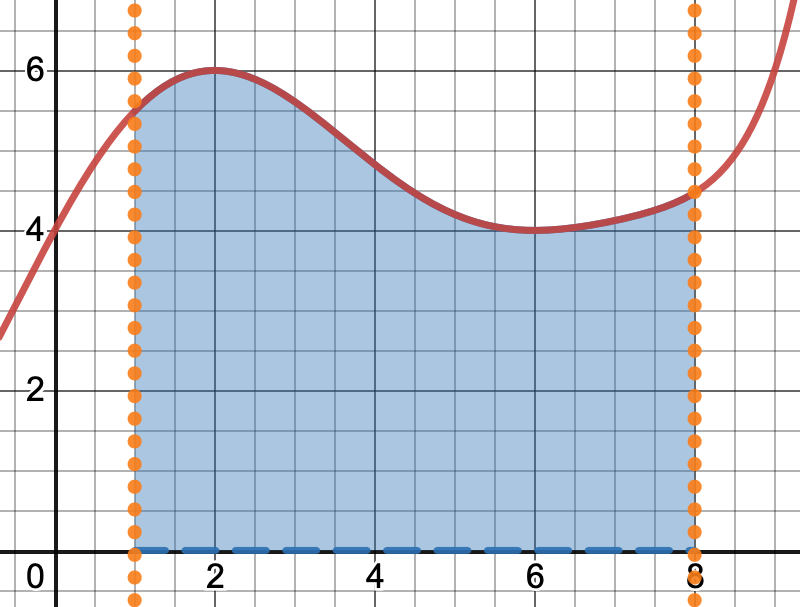
\includegraphics[width=8cm]{pic/areaunder.png}
\end{center}
\caption{Area below a graph}
\label{figareabelow}
\end{figure}
\begin{defn}
Consider the graph of a function $f\colon\R\to\R$ for $x$-values in an
interval $a\le x\le b$, as depicted in Figure~\ref{figareabelow} for $a=1$ and $b=8$. The value of the area enclosed by
\begin{itemize}
\item The $x$-axis,
\item the line $x=a$,
\item the line $x=b$, and
\item the graph of $f$.
\end{itemize}
is called the \defini{definite integral} of $f$ from $a$ to $b$ and denoted by
\[
\int_a^b f(x)\dm{x}.
\]
\end{defn}
Obviously there is no $+C$ in the definite integral -- the area is not subject to
choice.
\begin{note}
\label{defintprop}
For completeness, a few extra rules and observations on the definite integral are in order:
\begin{itemize}
\item If $a=b$ the area is zero: $\displaystyle\int_a^a f(x)\dm{x}=0$.
\item If $b<a$, we count the area negatively.
\item Similarly, if the function $f(x)\le 0$. The area above the $x$-axis is counted positively, the area below the $x$-axis negatively.
\item We can split an area by a vertical line $x=c$ into two parts, for $a\le c\le b$. Then
\[
\int_a^b f(x)\dm{x}= \int_a^c f(x)\dm{x}+ \int_c^b f(x)\dm{x}.
\]
the area is zero: $\displaystyle\int_a^a f(x)\dm{x}=0$.
\item
If we add two functions, we can split the area into two parts, using one of the
functions. That is
\[
\int_a^b f(x)+g(x)\dm{x}=\int_a^b f(x)\dm{x}+\int_a^b g(x)\dm{x}
\]
\end{itemize}
\end{note}

Besides the obvious geometric applications, we can use this area for example to define the \defini{average} of the function $f$ on the
interval from $a$ to $b$ as
\[
\frac{\int_a^b f(x)\dm{x}}{b-a}.
\]

\subsection{Riemann Sums}

While we can define the area under the graph, we have so far no general
formula from geometry to calculate it, unless $f$ has a very particular
form\mynote{say a straight line, or a half-circle}.

But we can approximate or estmate the area by covering it with smaller
pieces, whose area we can calculate. In the picture in
Figure~\ref{figareabelow}, the grid depicted helps with such an
approximation, giving an area between about 32 and 36 units\mynote{while the
correct area is about $33.7756$ units}.

While it seems clear that cutting in finer pieces will give a better result,
it is not clear how to do this cutting so that it will work for arbitrary
functions. The approach we shall employ, named \defini{Riemann
sums}\mynote{named after the German mathematician \textsc{Bernhard Riemann},
1826-1866} is
simple enough to allow for an easy description, while allowing for the
definiton of exact results: We split the area in vertical stripes of equal
width, such that the height of the stripe matches the function value on the
left side. Figure~\ref{figriemannsums} depicts such approximations for
$n=1,2,3,4,10,25$ stripes. The area of the stripes becomes a better and
better approximation of the area under the graph.

%https://www.desmos.com/calculator/m7cnldum8n
\begin{figure}
\begin{center}
\begin{tabular}{lll}
\begin{minipage}[t]{3.5cm}
1 rectangle: $38.43$\\
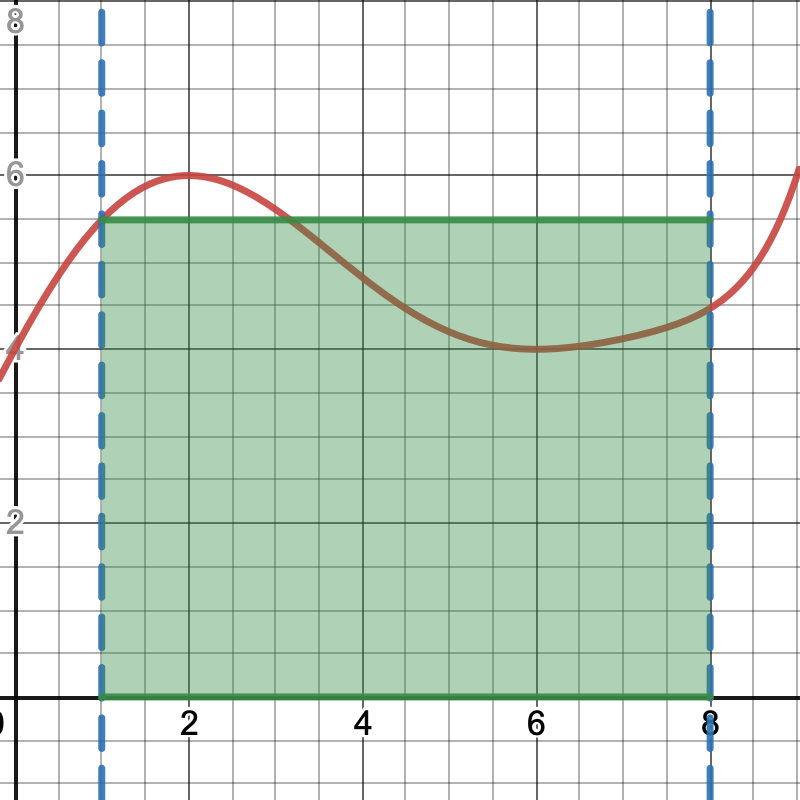
\includegraphics[width=3cm]{pic/riemannsum1.png}
\end{minipage}&\begin{minipage}[t]{3.5cm}
2 rectangles: $34.84$\\
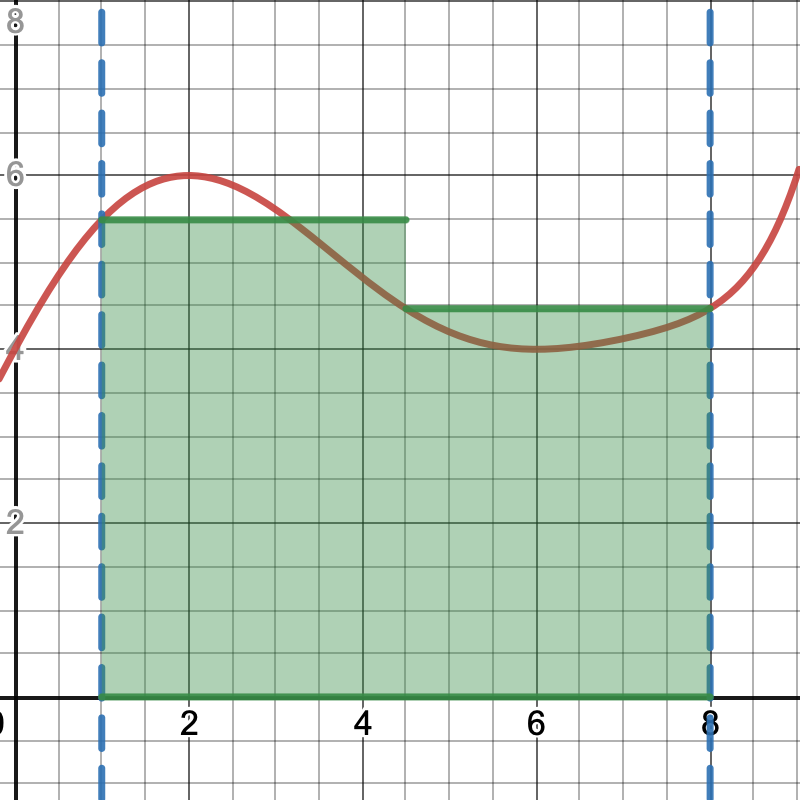
\includegraphics[width=3cm]{pic/riemannsum2.png}
\end{minipage}&\begin{minipage}[t]{3.5cm}
3 rectangles: $34.69$\\
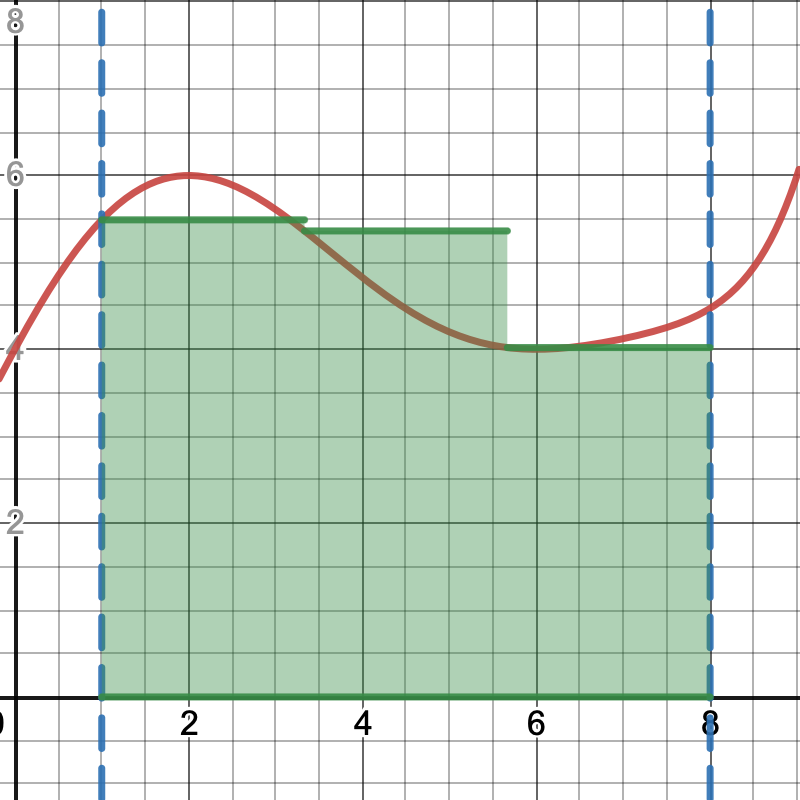
\includegraphics[width=3cm]{pic/riemannsum3.png}
\end{minipage}\\
\\
\begin{minipage}[t]{3.5cm}
4 rectangles: $34.53$\\
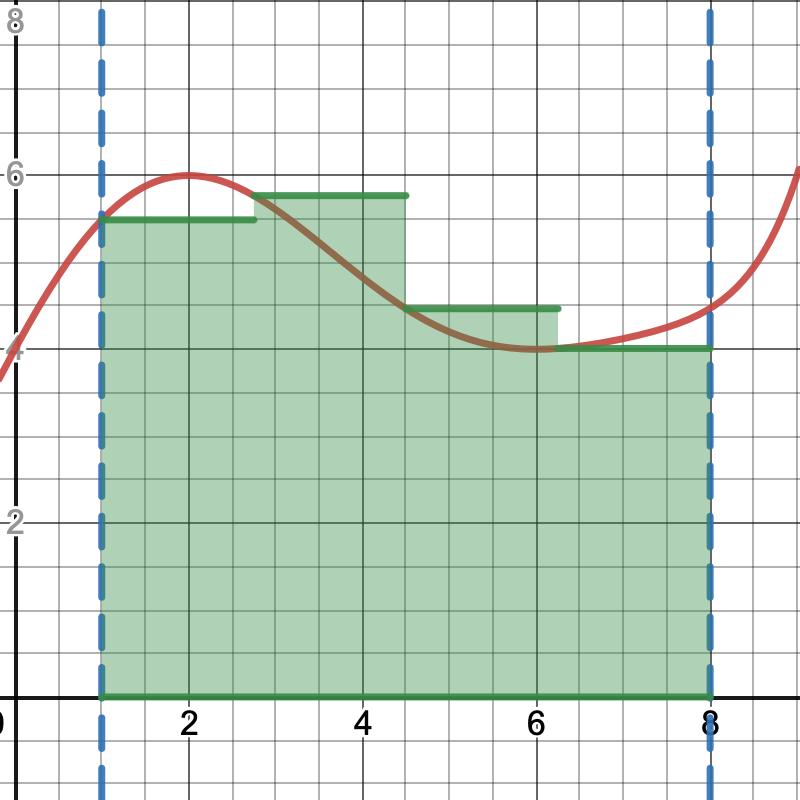
\includegraphics[width=3cm]{pic/riemannsum4.png}
\end{minipage}&\begin{minipage}[t]{3.5cm}
10 rectangles: $34.11$\\
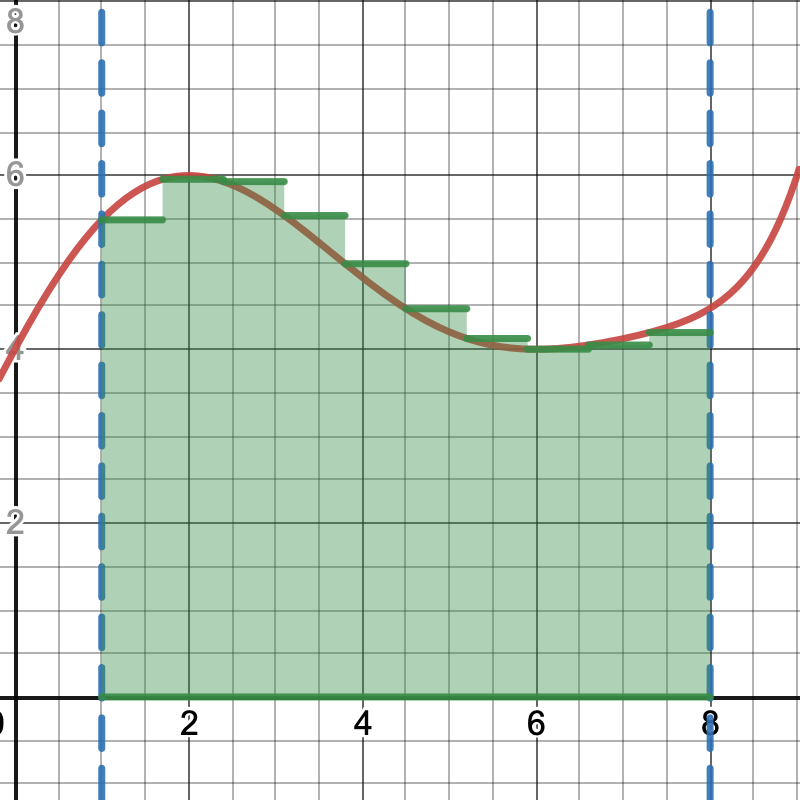
\includegraphics[width=3cm]{pic/riemannsum10.png}
\end{minipage}&\begin{minipage}[t]{3.5cm}
25 rectangles: $33.91$\\
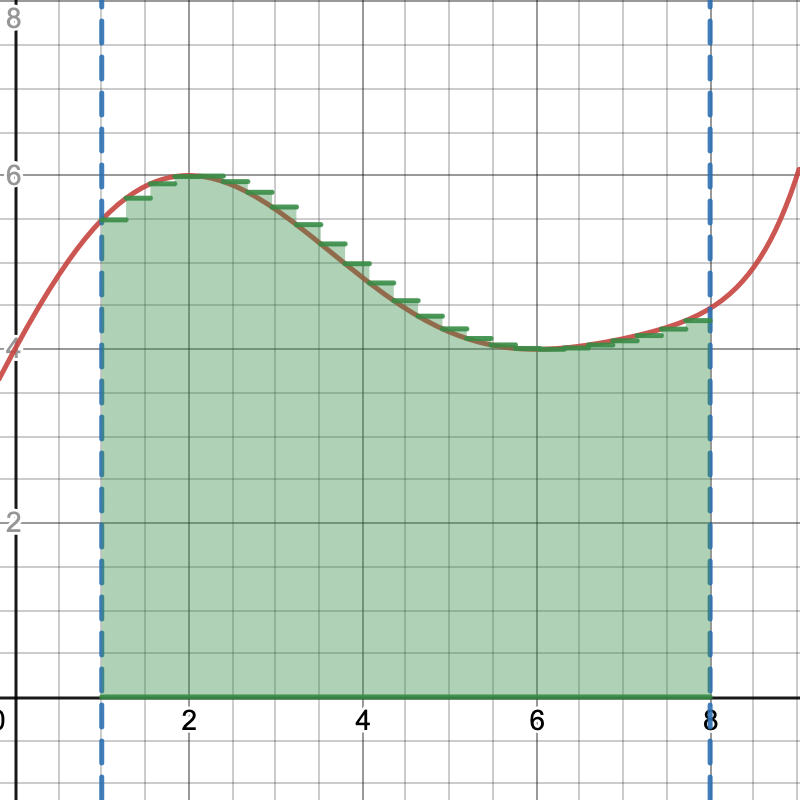
\includegraphics[width=3cm]{pic/riemannsum25.png}
\end{minipage}\\
\end{tabular}
\end{center}
\caption{Integral approximations by Riemann sums}
\label{figriemannsums}
\end{figure}

\begin{lemma}
\label{riemannarea}
If we split the interval into $k$ stripes of equal width, each stripe has
width $\Delta x=(b-a)/k$ and the $i$-th stripe starts at $x_i=a+(b-a)/k\cdot
(i-1)$. The total area of the $k$ stripes thus is
\[
A_k=\sum_{i=1}^k f(x_i)\cdot \Delta x
=\sum_{i=1}^k f\left(a+\frac{(b-a)(i-1)}{k}\right)\cdot\frac{b-a}{k}.
\]
\end{lemma}

In our example, (beyond the pictures shown), 100 intervals give us an area
of $33.81$, 200 intervals give $33.79$, 1000 intervals $33.779$, and 10000
intervals $33.7759$.

\begin{note}
The decision to set the height of a stripe at the function value on the left side does
not necessarily give the best approximation. Others options are right
side, middle, or largest or smallest value of the function in the interval.
Indeed such different strategies are all used if one wants to approximate the
area numerically. For our purposes however the difference between these
methods is irrelevant, as we aim to make the stripes infinitesimally narrow.
\end{note}

We note that, unsurprisingly, a choice of finer and finer stripes gives an
increasingly better approximation of the area. Indeed, one can show if we
consider the values of the stripe approximations $A_k$ as a sequence,
$(A_k)$, indexed by $k$, that this sequence converges in our example.

\begin{defn}
\label{defdefn}
More generally, we call a function \defini{integrable} on the interval from
$a$ to $b$, if the limit
\[
\lim_{k\to\infty} A_k
\]
exists (and is finite). This is for example the case if $f$ is continuous.
And the value of the definite integral then is defined as this limit:
\[
\int_a^b f(x)\dm{x}=\lim_{k\to\infty} A_k.
\]
\end{defn}
\begin{note}
The summation formula in Lemma~\ref{riemannarea} is the origin for the integral
notation. The $\sum$ is transformed in a lengthy ``S'', the integral sign
$\int$, and the interval width $\Delta x$ becomes the end delimiter
$\dm{x}$.
\end{note}

\begin{note}
The reader might worry that we now defined the definite integral twice -- once as
area, and once as limit. Indeed, the proper approach would be to define the
improper integral as a limit as in definition~\ref{defdefn}, show that it obeys
the properties, in particular the area aditivity of Note~\ref{defintprop}, and
show that in cases that a graph defines an area that is a geometric object defined
in school, the geometric area, and the value of the improper integral agree. Doing
so is not particularly illustrative, and thus we do not do so here.
For areas that were never calculated in geometry class, the definite integral then
{\em is} the definition of their area.
\end{note}

\section{The Fundamental Theorem}

The definition of the definite integral as a limit is not particularly helpful to
calculating it. We thus instead use another approach that will lead us to a
connection with antiderivatives.

For this, assume now that $f(x)$ is an integrable function.
We define a new function that gives values of certain definite integrals:
\[
F(z)=\int_0^z f(x)\dm{x}.
\]
(The choice of $0$ is arbitrary, one could chose any other number instead.)
Note that we need to call the integration variable (here $x$) differently from $z$
to avoid confusion of variables.

That is, the function $F$ assigns to every number $z$ the value of the definite
integral from $0$ to $z$ over the function $f$; that is the area under the graph
of $f$ from $0$ to $z$.

We now consider how $F(z)$ changes when $z$ changes:
\begin{thm}[Fundamental Theorem of Calculus]\ \\
a)The function $F(z)$ is differentiable with respect to the variable $z$, and we
have that
\[
\frac{\dm{}}{\dm{z}} F(z)=f(z),
\]
that is $F(x)$ is an antiderivative of $f(x)$.\\
b) For any $a,b\in\R$, we have that 
\[
\int_a^b f(x)\dm{x}=F(b)-F(a).
\]
c) If $G$ is {\em any} antiderivative of $f$, we have that
\[
\int_a^b f(x)\dm{x}=G(b)-G(a).
\]
\end{thm}
To show the connection and to save space, we write $\displaystyle
F(x)\biggm|_a^b=F(b)-F(a)$.
\begin{proof}
a) We use the definition of the derivative as limit of the difference quotient:
\[
\frac{\dm{}}{\dm{x}} F(x)=\lim_{h\to 0}\frac{F(x+h)-F(x)}{h}
\]
The difference in the numerator is the difference of the two areas, as depicted in
green in Figure~\ref{figfundthm}. 
\begin{figure}
\begin{center}
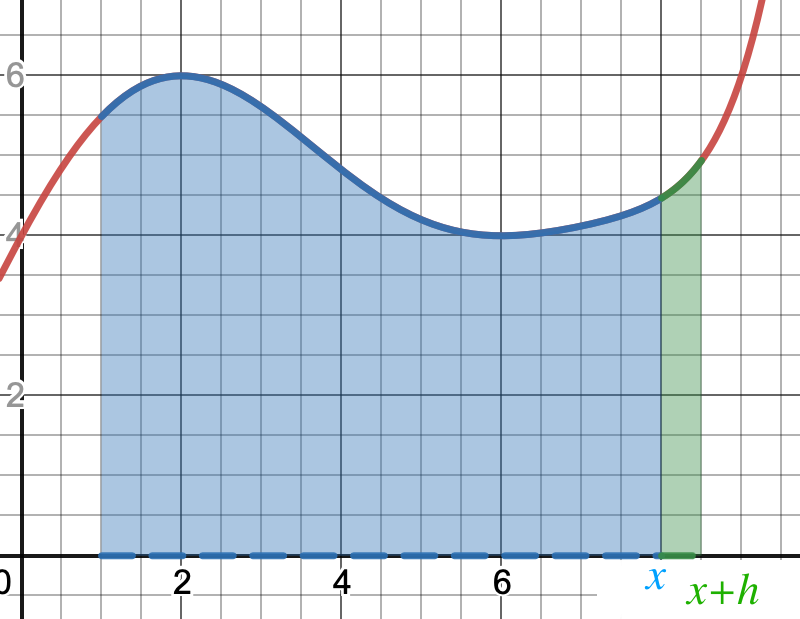
\includegraphics[width=6cm]{pic/fundthm.png}
\end{center}
\caption{Proof of the Fundamental Theorem}
\label{figfundthm}
\end{figure}
As $h\to 0$, this area is apprixmated by a single vertical strip of width $h$ and
height $f(x)$, and thus area $f(x)\cdot h$. The quotient thus has the limit
$f(x)$.\\
b) By the rules for additivity of area, we have that
\[
\int_a^b f(x)\dm{x}=\int_0^b f(x)\dm{x}-\int_0^a f(x)\dm{x}=F(b)-F(a).
\]
c) If $G(x)$ is another antiderivative, we have that $G(x)=F(x)+c$ for some
constant $c$. But then
\[
G(b)-G(a)=F(b)+c-(F(a)+c)=F(b)-F(a)+c-c=F(b)-F(a)=\int_a^b f(x)\dm{x}.
\]
\end{proof}
\begin{bsp}
\[
\int_0^\pi
\sin(x)\dm{x}=(-\cos(x))\biggm|_0^\pi=-\cos(\pi)-(-\cos(0))=-(-1)-(-1)=2
\]
and (verify the antiderivative by differentiation!)
\[
\int_{-1}^1\sqrt{1-x^2}\dm{x}=\left(\frac12\left(x\sqrt{1-x^2}+\arcsin(x)\right)\right)
\biggm|_{-1}^1=\frac12(\pi/2-(-\pi/2))=\frac{\pi}{2}
\]
the area of a half-circle (thus verifying the circle-area formula from school).
\end{bsp}

Some examples of applications of definite integrals are:
\paragraph{Areas and Volumes}
If we can describe an regions using functions, we can often use integrals to calculate their areas. Building on this we can calculate not
only the volumes of prisms (area of the base times height), but also volumes of objects that can be built from areas in a regular way --
pyramids and cones, or volumes obtained by rotating a region throuigh higher dimensional space.
\paragraph{Averages}
We have already seen that one can define an ``average'' value of a function over an interval as the quotient of the definite integral by
the interval length. In similar way one can calculate other statistical measures, determine centers of mass, or renormalize functions to
make them comparable.
\paragraph{Infinite summations}
The definition of definite integrals is as limit of a sum. There are other measures that can be described as such a limit -- for example
the length of a curve, or a more compiclated surface area, and the limit expression then can be interpreted as a definite integral.
\paragraph{Geometry on Functions}
What is probably the most important application of definite integrals for
computer science might also initialy seem the most cryptic one. You will see
in Linear Algebra classes, that definite integrals can be used to define an
``length'' of functions on an interval $[a,b]$. Concretely, the length of
the functions $f$ can be defined as
\[
\sqrt{
\int_a^b f(x)^2\dm{x}}
\]
Using the concept of length, it is possible to continue in defining angles,
orthogonality, projections, close approximations, and ultimately use the
tools of geometry to investigate functions.


